% \documentclass{article}
% \usepackage[utf8]{inputenc}
% \usepackage{tikz}
% \begin{document}

\centering
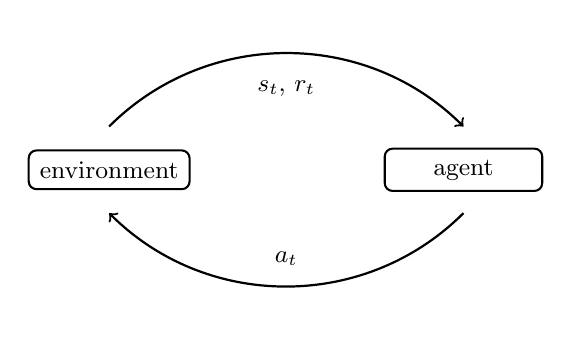
\begin{tikzpicture}[
  % GLOBAL CFG
  % font=\sf \scriptsize,
  % Styles
  cell/.style={% For the main box
      rectangle, 
      rounded corners=5mm, 
      draw,
      very thick,
      },
  operator/.style={%For operators like +  and  x
      circle,
      draw,
      inner sep=-0.5pt,
      minimum height =.4cm,
      },
  function/.style={%For functions
      ellipse,
      draw,
      inner sep=1pt
      },
  ct/.style={% For external inputs and outputs
      rectangle, 
      rounded corners=1mm, 
      draw,
      line width = .75pt,
      minimum width=1cm,
      inner sep=4pt,
      },
  gt/.style={% For internal inputs
      rectangle,
      draw,
      minimum width=10mm,
      minimum height=6mm,
      inner sep=1pt
      },
  empty/.style={% Empty nodes for joining arrows
      rectangle,
      draw,
      minimum width=0mm,
      minimum height=0mm,
      inner sep=0pt
      },
  mylabel/.style={% something new that I have learned
      font=\scriptsize\sffamily
      },
  ArrowC1/.style={% Arrows with rounded corners
      rounded corners=.25cm,
      thick,
      },
  ArrowC2/.style={% Arrows with big rounded corners
      rounded corners=.5cm,
      thick,
      },
  ]
    
    %Start drawing the thing...    

  % Draw the cell: 
  % \node [cell, minimum height =1cm, minimum width=3cm] at (0,0){\small Environment} ;
  % \node [cell, minimum height =1cm, minimum width=3cm] at (4.5,0){\small Agent} ;


  \node [ct, minimum width=2cm] (optim1) at (0,0) {\small environment}; 
  \node [ct, minimum width=2cm] (optim1) at (4.5,0) {\small agent}; 

  \node [empty, label={\small $a_t$}] (action) at (2.25, -1.35) {};
  \node [empty, label={\small $s_t$, $r_t$}] (state) at (2.25, 0.8) {};

  \draw [->, thick] (0, 0.55) to[out=45,in=135] (4.5, 0.55);
  \draw [->, thick] (4.5, -0.55) to[out=-135,in=-45] (0, -0.55);
  


\end{tikzpicture}

% \end{document}
